\documentclass[notes,11pt, aspectratio=169]{beamer}

\usepackage{pgfpages}
% These slides also contain speaker notes. You can print just the slides,
% just the notes, or both, depending on the setting below. Comment out the want
% you want.
\setbeameroption{hide notes} % Only slide
%\setbeameroption{show only notes} % Only notes
%\setbeameroption{show notes on second screen=right} % Both

\usepackage{helvet}
\usepackage[default]{lato}
\usepackage{array}
\usepackage{tgbonum}

\usepackage{tikz}
\usepackage{verbatim}
\setbeamertemplate{note page}{\pagecolor{yellow!5}\insertnote}
\usetikzlibrary{positioning}
\usetikzlibrary{snakes}
\usetikzlibrary{calc}
\usetikzlibrary{arrows}
\usetikzlibrary{decorations.markings}
\usetikzlibrary{shapes.misc}
\usetikzlibrary{matrix,shapes,arrows,fit,tikzmark}
\usepackage{amsmath}
\usepackage{mathpazo}
\usepackage{hyperref}
\usepackage{lipsum}
\usepackage{multimedia}
\usepackage{graphicx}
\usepackage{multirow}
\usepackage{graphicx}
\usepackage{dcolumn}
\usepackage{bbm}
\newcolumntype{d}[0]{D{.}{.}{5}}

\usepackage{changepage}
\usepackage{appendixnumberbeamer}
\newcommand{\beginbackup}{
   \newcounter{framenumbervorappendix}
   \setcounter{framenumbervorappendix}{\value{framenumber}}
   \setbeamertemplate{footline}
   {
     \leavevmode%
     \hline
     box{%
       \begin{beamercolorbox}[wd=\paperwidth,ht=2.25ex,dp=1ex,right]{footlinecolor}%
%         \insertframenumber  \hspace*{2ex}
       \end{beamercolorbox}}%
     \vskip0pt%
   }
 }
\newcommand{\backupend}{
   \addtocounter{framenumbervorappendix}{-\value{framenumber}}
   \addtocounter{framenumber}{\value{framenumbervorappendix}}
}


\usepackage{graphicx}
\usepackage[space]{grffile}
\usepackage{booktabs}
\newcommand\independent{\protect\mathpalette{\protect\independenT}{\perp}}
\def\independenT#1#2{\mathrel{\rlap{$#1#2$}\mkern2mu{#1#2}}}
\DeclareMathOperator{\Supp}{Supp}

% These are my colors -- there are many like them, but these ones are mine.
\definecolor{blue}{RGB}{0,114,178}
\definecolor{red}{RGB}{213,94,0}
\definecolor{yellow}{RGB}{240,228,66}
\definecolor{green}{RGB}{0,158,115}

\hypersetup{
  colorlinks=false,
  linkbordercolor = {white},
  linkcolor = {blue}
}


%% I use a beige off white for my background
\definecolor{MyBackground}{RGB}{255,253,218}

%% Uncomment this if you want to change the background color to something else
%\setbeamercolor{background canvas}{bg=MyBackground}

%% Change the bg color to adjust your transition slide background color!
\newenvironment{transitionframe}{
  \setbeamercolor{background canvas}{bg=yellow}
  \begin{frame}}{
    \end{frame}
}

\setbeamercolor{frametitle}{fg=blue}
\setbeamercolor{title}{fg=black}
\setbeamertemplate{footline}[frame number]
\setbeamertemplate{navigation symbols}{}
\setbeamertemplate{itemize items}{-}
\setbeamercolor{itemize item}{fg=blue}
\setbeamercolor{itemize subitem}{fg=blue}
\setbeamercolor{enumerate item}{fg=blue}
\setbeamercolor{enumerate subitem}{fg=blue}
\setbeamercolor{button}{bg=MyBackground,fg=blue,}



% If you like road maps, rather than having clutter at the top, have a roadmap show up at the end of each section
% (and after your introduction)
% Uncomment this is if you want the roadmap!
% \AtBeginSection[]
% {
%    \begin{frame}
%        \frametitle{Roadmap of Talk}
%        \tableofcontents[currentsection]
%    \end{frame}
% }
\setbeamercolor{section in toc}{fg=blue}
\setbeamercolor{subsection in toc}{fg=red}
\setbeamersize{text margin left=1em,text margin right=1em}

\newenvironment{wideitemize}{\itemize\addtolength{\itemsep}{10pt}}{\enditemize}

\usepackage{environ}
\NewEnviron{videoframe}[1]{
  \begin{frame}
    \vspace{-8pt}
    \begin{columns}[onlytextwidth, T] % align columns
      \begin{column}{.70\textwidth}
        \begin{minipage}[t][\textheight][t]
          {\dimexpr\textwidth}
          \vspace{8pt}
          \hspace{4pt} {\Large \sc \textcolor{blue}{#1}}
          \vspace{8pt}

          \BODY
        \end{minipage}
      \end{column}%
      \hfill%
      \begin{column}{.38\textwidth}
        \colorbox{green!20}{\begin{minipage}[t][1.2\textheight][t]
            {\dimexpr\textwidth}
            Face goes here
          \end{minipage}}
      \end{column}%
    \end{columns}
  \end{frame}
}

\title[]{\textcolor{blue}{Canonical Research Designs I:\\ Difference-in-Differences:\\ Extensions and Alternatives}}
\author[PGP]{}
\institute[FRBNY]{\small{\begin{tabular}{c}
  Paul Goldsmith-Pinkham  \\
\end{tabular}}}

\date{\today}

\begin{document}

%%% TIKZ STUFF
\tikzset{
        every picture/.style={remember picture,baseline},
        every node/.style={anchor=base,align=center,outer sep=1.5pt},
        every path/.style={thick},
        }
\newcommand\marktopleft[1]{%
    \tikz[overlay,remember picture]
        \node (marker-#1-a) at (-.3em,.3em) {};%
}
\newcommand\markbottomright[2]{%
    \tikz[overlay,remember picture]
        \node (marker-#1-b) at (0em,0em) {};%
}
\tikzstyle{every picture}+=[remember picture]
\tikzstyle{mybox} =[draw=black, very thick, rectangle, inner sep=10pt, inner ysep=20pt]
\tikzstyle{fancytitle} =[draw=black,fill=red, text=white]
%%%% END TIKZ STUFF

% Title Slide
\begin{frame}
\maketitle
\end{frame}

%% Synthetic Control block (from 14_synthetic_dind.tex)

\begin{frame}{Generalizing the Dind approach }
  \begin{columns}[T] % align columns
    \begin{column}{0.9\textwidth}
      \begin{wideitemize}
      \item Pivoting slightly: instead of imposing the parallel trends
        assumption directly through the linear model, we could
        construct a combination of units to approximate $Y_{it}(0)$
        \begin{itemize}
        \item This is what one does in the cross-sectional setting with a
          pscore method! E.g. consider the ATT:
          \begin{equation*}
            \tau_{ATT} = \underbrace{Y(1)}_{\text{Fully observed}} - \underbrace{\hat{Y}(0)}_{\text{Constructed}}
          \end{equation*}
        \end{itemize}
      \item How would one pick? Recall that with p-score methods or
        regression, weights effectively reweight based on
        comparability to treated group
        \begin{itemize}
        \item With panel data, can use pre-treatment data to construct
          these weights
        \item This method is known as synthetic control (and its various descendents)
        \end{itemize}
      \end{wideitemize}
    \end{column}%
    \hfill%
    \begin{column}{.5\textwidth}
    \end{column}%
  \end{columns}
\end{frame}


\begin{frame}{Synthetic Control example - (Abadie et al. (2010)) }
  \begin{columns}[T] % align columns
    \begin{column}{0.5\textwidth}
      \begin{wideitemize}
      \item Consider following problem: California bans smoking in 1989. What does that do to smoking?
        \begin{itemize}
        \item Define estimand: $\tau_{ban,CA} = Y_{california, post}(1) - Y_{california, post}(0)$
        \item This is the effect of the \emph{California} smoking ban
        \item How can we get at it?
        \end{itemize}
      \item We need a ``synthetic California'' as our control
      \item In an ideal world, the average of the other states would
        work -- however, not clear empirically that they are a good
        counterfactual
      \end{wideitemize}
    \end{column}%
    \hfill%
    \begin{column}{.5\textwidth}
      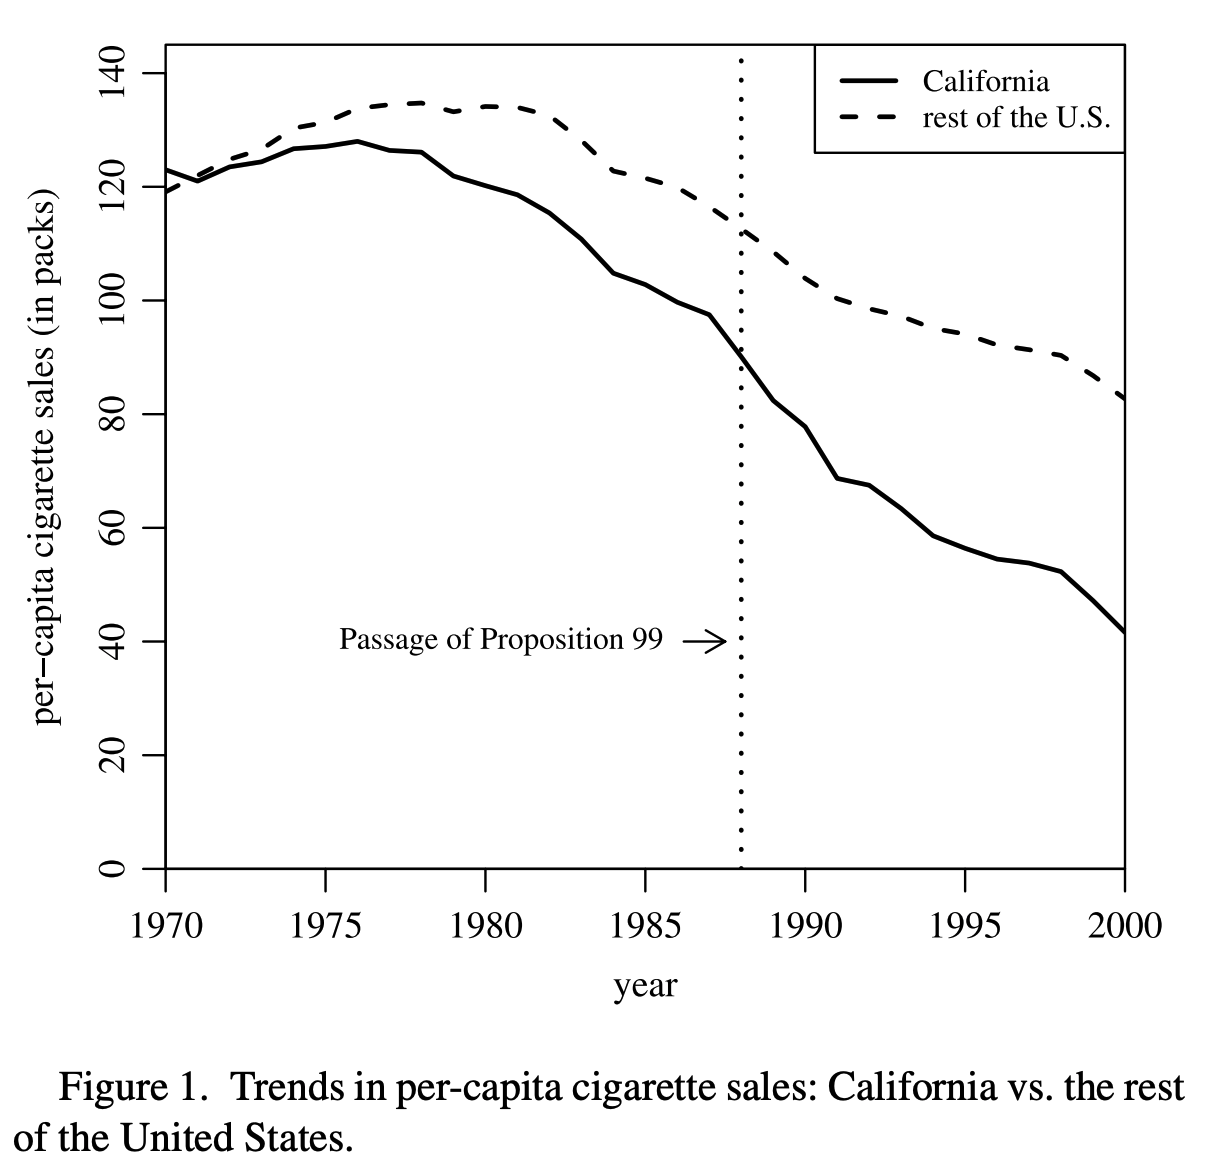
\includegraphics[width=\linewidth]{images/abadie2010a.png}
    \end{column}%
  \end{columns}
\end{frame}


\begin{frame}{Generalized setup (Doudchenko and Imbens (2018))}
  \begin{wideitemize}
  \item Consider the following general problem
    \item We have a panel with $T$ time periods and $N+1$
      units. Intervention $D_{it}$ at time $T_{0}$ for one unit (unit $i = 0$)
    \item Potential outcomes $Y_{it}(D_{it})$, and we only observe one
      of the potential outcomes (as per usual)
      \begin{itemize}
      \item Fundamental problem of causal inference
      \item We can also have fixed characteristics $X_{it}$
      \end{itemize}
    \item Let $\mathbf{Y}_{a,b}$ denote the vector (or matrix in
      control case) for $a \in \{\text{treatment}, \text{control}\}$ and
      $b \in \{\text{pre}, \text{post}\}$ for the treated and control
      groups in the pre or post period.
    \item Then, we have observations (analogous setup for the covariates):
      \begin{equation*}
        \mathbf{Y} = \left( \begin{array}{cc}
                              \mathbf{Y}_{t,post} & \mathbf{Y}_{c,post} \\
                              \mathbf{Y}_{t,pre} & \mathbf{Y}_{c,pre} \\
                            \end{array}
                            \right) =  \left( \begin{array}{cc}
                              \mathbf{Y}_{t,post}(1) & \mathbf{Y}_{c,post}(0) \\
                              \mathbf{Y}_{t,pre}(0) & \mathbf{Y}_{c,pre}(0) \\
                            \end{array}
                            \right)
      \end{equation*}
  \end{wideitemize}
\end{frame}

\begin{frame}{Generalized panel setup}
      \begin{equation*}
        \mathbf{Y} = \left( \begin{array}{cc}
                              \mathbf{Y}_{t,post} & \mathbf{Y}_{c,post} \\
                              \mathbf{Y}_{t,pre} & \mathbf{Y}_{c,pre} \\
                            \end{array}
                            \right) =  \left( \begin{array}{cc}
                              \mathbf{Y}_{t,post}(1) & \mathbf{Y}_{c,post}(0) \\
                              \mathbf{Y}_{t,pre}(0) & \mathbf{Y}_{c,pre}(0) \\
                            \end{array}
                            \right)
      \end{equation*}
      \begin{wideitemize}
      \item To estimate $\tau_{i} = Y_{t,post}(1) - Y_{t,post}(0)$, we
        need an estimate for $Y_{t,post}(0)$
      \item What if we just had the cross-section?
        \begin{itemize}
        \item Note that if $D_{it}$ were randomly assigned, we can
          derive an estimate using our p-score or regression methods
        \item Even without random assignment, one could use covariates
          to match
        \item Our main concern with p-score matching is bias
        \end{itemize}
      \item Diff-in-diff exploited the panel structure by asserting a particular functional form
        \begin{equation*}
          Y_{it} = \alpha_{i} + \gamma_{t} + D_{it}\tau + \epsilon_{it}
        \end{equation*}
      \item Is there something particularly special about this linear
        additive factor structure?
      \end{wideitemize}
\end{frame}


\begin{frame}{Generalized panel setup}
      \begin{equation*}
        \mathbf{Y} = \left( \begin{array}{cc}
                              \mathbf{Y}_{t,post} & \mathbf{Y}_{c,post} \\
                              \mathbf{Y}_{t,pre} & \mathbf{Y}_{c,pre} \\
                            \end{array}
                            \right) =  \left( \begin{array}{cc}
                              \mathbf{Y}_{t,post}(1) & \mathbf{Y}_{c,post}(0) \\
                              \mathbf{Y}_{t,pre}(0) & \mathbf{Y}_{c,pre}(0) \\
                            \end{array}
                            \right)
      \end{equation*}
      \begin{wideitemize}
      \item Recall that our problem boils down to the estimate of an untreated ``synthetic'' unit
      \item Following Doudchenko and Imbens (2018), note estimators of the following form:
        \begin{equation*}
          \hat{Y}_{t,post}(0) = \mu + \sum_{i \in c}\omega_{i} Y_{i, T}
        \end{equation*}
        \begin{itemize}
        \item A constant $\mu$ allows for very different averages (common in diff-in-diff)
        \item Weights are allowed to vary across $i$ -- a simple
          average would be diff-in-diff
        \end{itemize}
      \item We can now consider deviations from diff-in-diff
      \end{wideitemize}
\end{frame}

\begin{frame}{The synthetic control method (Abadie et al. (2010)}
  \begin{columns}[T] % align columns
    \begin{column}{0.8\textwidth}
  \begin{equation*}
    \hat{Y}_{t,post}(0) = \mu + \sum_{i \in c}\omega_{i} Y_{i, T}
  \end{equation*}
  \begin{wideitemize}
  \item In ADH, they impose
    \begin{enumerate}
    \item $\mu = 0$
    \item $\sum_{i} \omega_{i} = 1$
    \item $\omega_{i} \geq 0 \; \forall i$
    \end{enumerate}
  \item These three restrictions create a counterfactual California
    whose outcomes are within the support of the other states, and
    is a weighted sum of a subset of states
  \end{wideitemize}
\end{column}
\begin{column}{0.4\textwidth}
\end{column}
\end{columns}
\end{frame}

\begin{frame}{The synthetic control method (Abadie et al. (2010)}
  \begin{columns}[T] % align columns
    \begin{column}{0.8\textwidth}
  \begin{equation*}
    \hat{Y}_{t,post}(0) = \mu + \sum_{i \in c}\omega_{i} Y_{i, T}
  \end{equation*}
  \begin{wideitemize}
  \item Formally, the $\omega_{i}$ need to be estimated, and are
    constructed by minimizing the distance between covariates in the pre-period:
    \begin{equation*}
      ||\boldsymbol{X}_{\text{treat}} - \boldsymbol{X}_{\text{control}}\boldsymbol{W}||
    \end{equation*}
  \item The crucial piece tying this together: $\boldsymbol{X}$ can
    include both lagged outcomes, and covariates.
  \item Note we can now re-envision our panel data:
    \begin{itemize}
    \item Observed outcomes:     $\mathbf{Y}_{t,post}(1)$, $\mathbf{Y}_{c,post}(0)$
    \item Observed covariates / predictors: $\mathbf{Y}_{t,pre}(0)$, $\mathbf{Y}_{c,pre}(0)$, $\mathbf{X}_{t}$, $\mathbf{X}_{c}$
    \end{itemize}
  \item In many ways, this is just a matching problem using many characteristics!
  \end{wideitemize}
\end{column}
\begin{column}{0.4\textwidth}
\end{column}
\end{columns}
\end{frame}

\begin{frame}{The synthetic control method (Abadie et al. (2010)}
  \begin{columns}[T] % align columns
    \begin{column}{0.9\textwidth}
  \begin{equation*}
    \hat{Y}_{t,post}(0) = \mu + \sum_{i \in c}\omega_{i} Y_{i, T}
  \end{equation*}
  \begin{wideitemize}
  \item Formally, the $\omega_{i}$ need to be estimated, and are
    constructed by minimizing the distance between covariates in the pre-period:
    \begin{equation*}
      \{\hat{\omega} \}_{i} = \arg\min_{\boldsymbol{W}}||\boldsymbol{X}_{\text{treat}} - \boldsymbol{X}_{\text{control}}\boldsymbol{W}||
    \end{equation*}
  \item The crucial piece tying this together: $\boldsymbol{X}$ can
    include both lagged outcomes, and covariates.
  \item Note we can now re-envision our panel data:
    \begin{itemize}
    \item Observed outcomes:     $\mathbf{Y}_{t,post}(1)$, $\mathbf{Y}_{c,post}(0)$
    \item Observed covariates / predictors: $\mathbf{Y}_{t,pre}(0)$, $\mathbf{Y}_{c,pre}(0)$, $\mathbf{X}_{t}$, $\mathbf{X}_{c}$
    \end{itemize}
  \item In many ways, this is just a matching problem using many characteristics!
  \end{wideitemize}
\end{column}
\begin{column}{0.4\textwidth}
\end{column}
\end{columns}
\end{frame}

\begin{frame}{The synthetic control method (Abadie et al. (2010)}
  \begin{columns}[T] % align columns
    \begin{column}{0.5\textwidth}
  \begin{wideitemize}
  \item<1-> This approach can be incredibly successful
  \item<2-> By careful construction of a synthetic control, can
    calculate counterfactual impacts due to policy
  \item<2-> Still subject to same caveats from DinD -- not invariant
    to some transformations (e.g. log and linear)
  \end{wideitemize}
\end{column}
\begin{column}{0.5\textwidth}
  \only<1>{  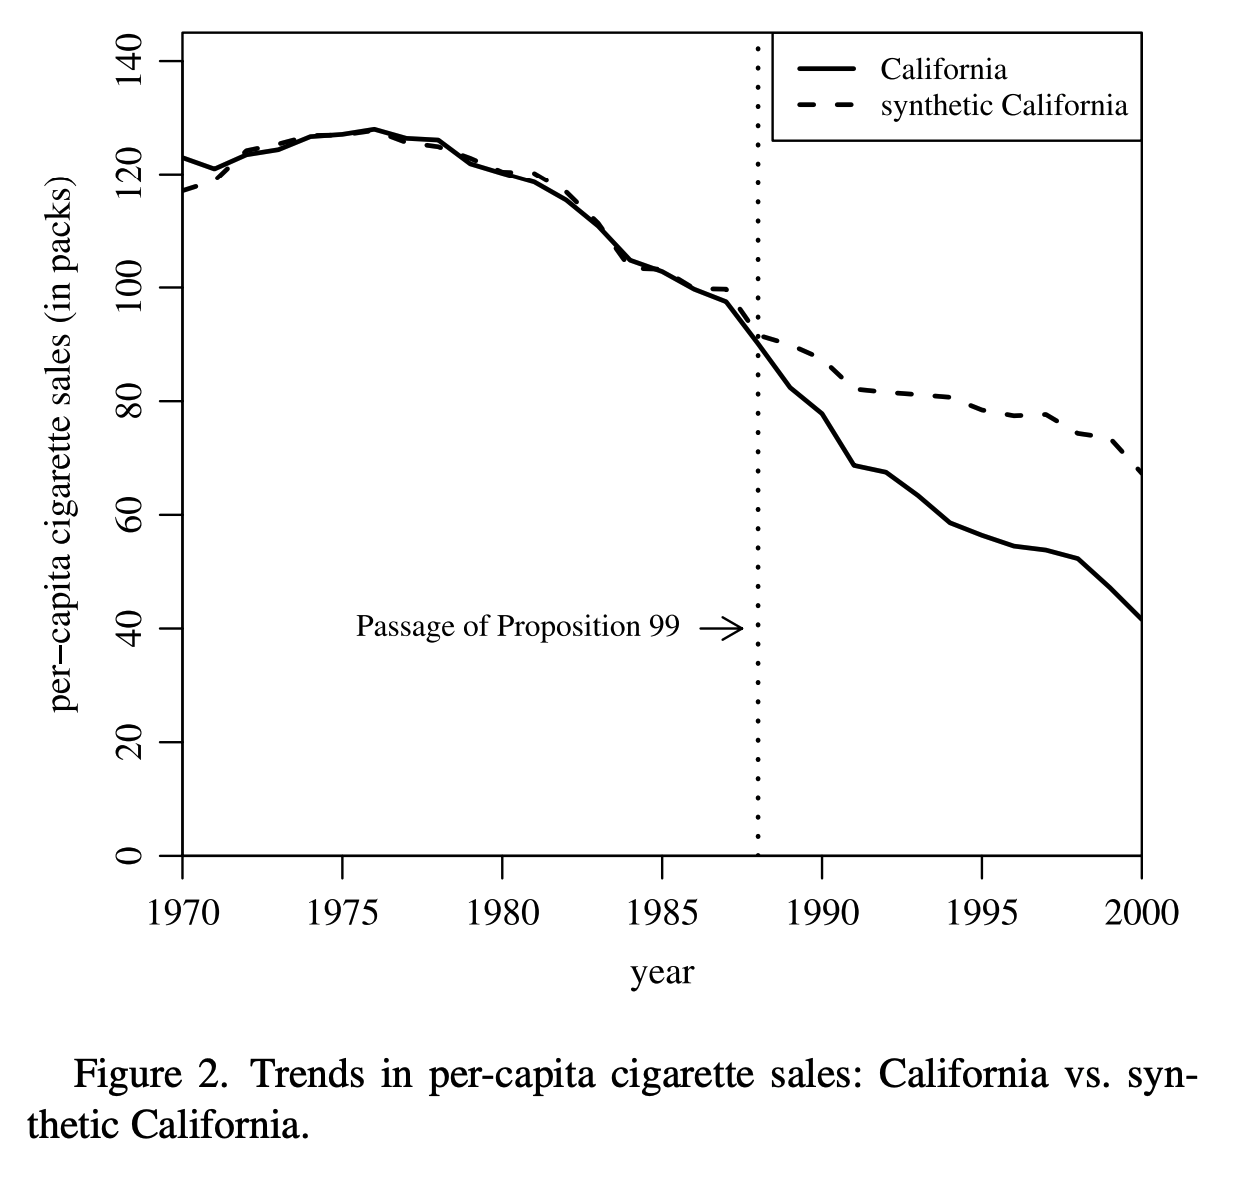
\includegraphics[width=\linewidth]{images/abadie2010b.png}}
\only<2>{  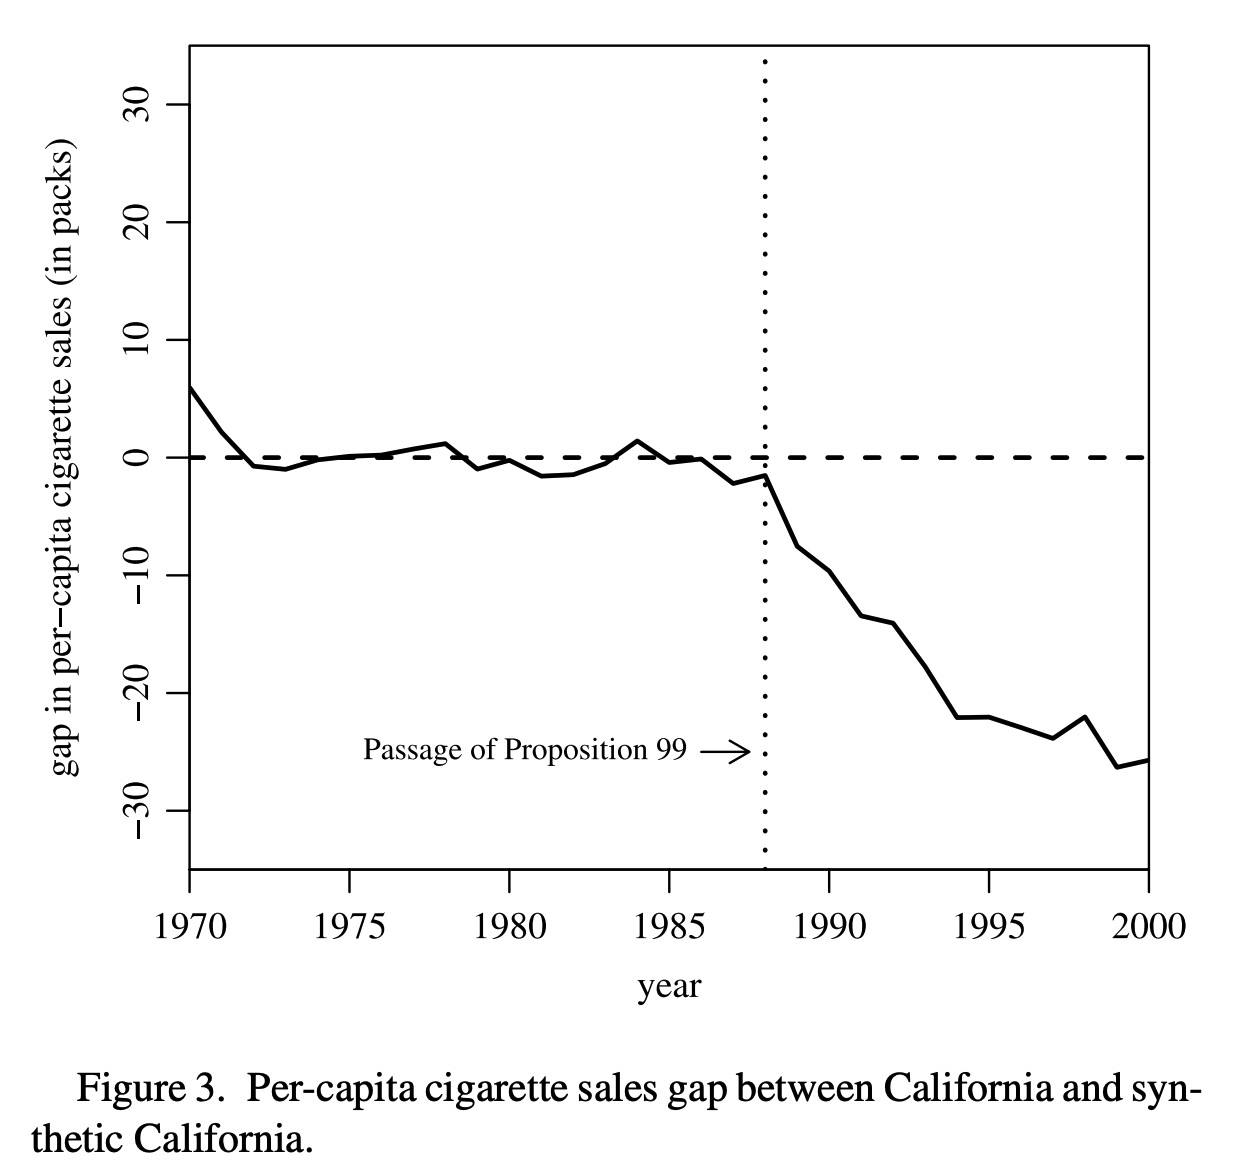
\includegraphics[width=\linewidth]{images/abadie2010c.png}}
\end{column}
\end{columns}
\end{frame}


\begin{frame}{Inference in the synthetic control method (Abadie et al. (2010)}
  \begin{columns}[T] % align columns
    \begin{column}{0.5\textwidth}
  \begin{wideitemize}
  \item Inference for this method is slightly more complex, as there
    is only a single treated unit
    \begin{itemize}
    \item Large sample asymptotics unlikely to work
    \end{itemize}
  \item Placebo approach is standard: apply method to each potential
    control unit, and report effect in period
  \item Analogy here is to a randomization inference argument,
    comparing to a ``null'' effect
  \end{wideitemize}
\end{column}
\begin{column}{0.5\textwidth}
  \only<1>{  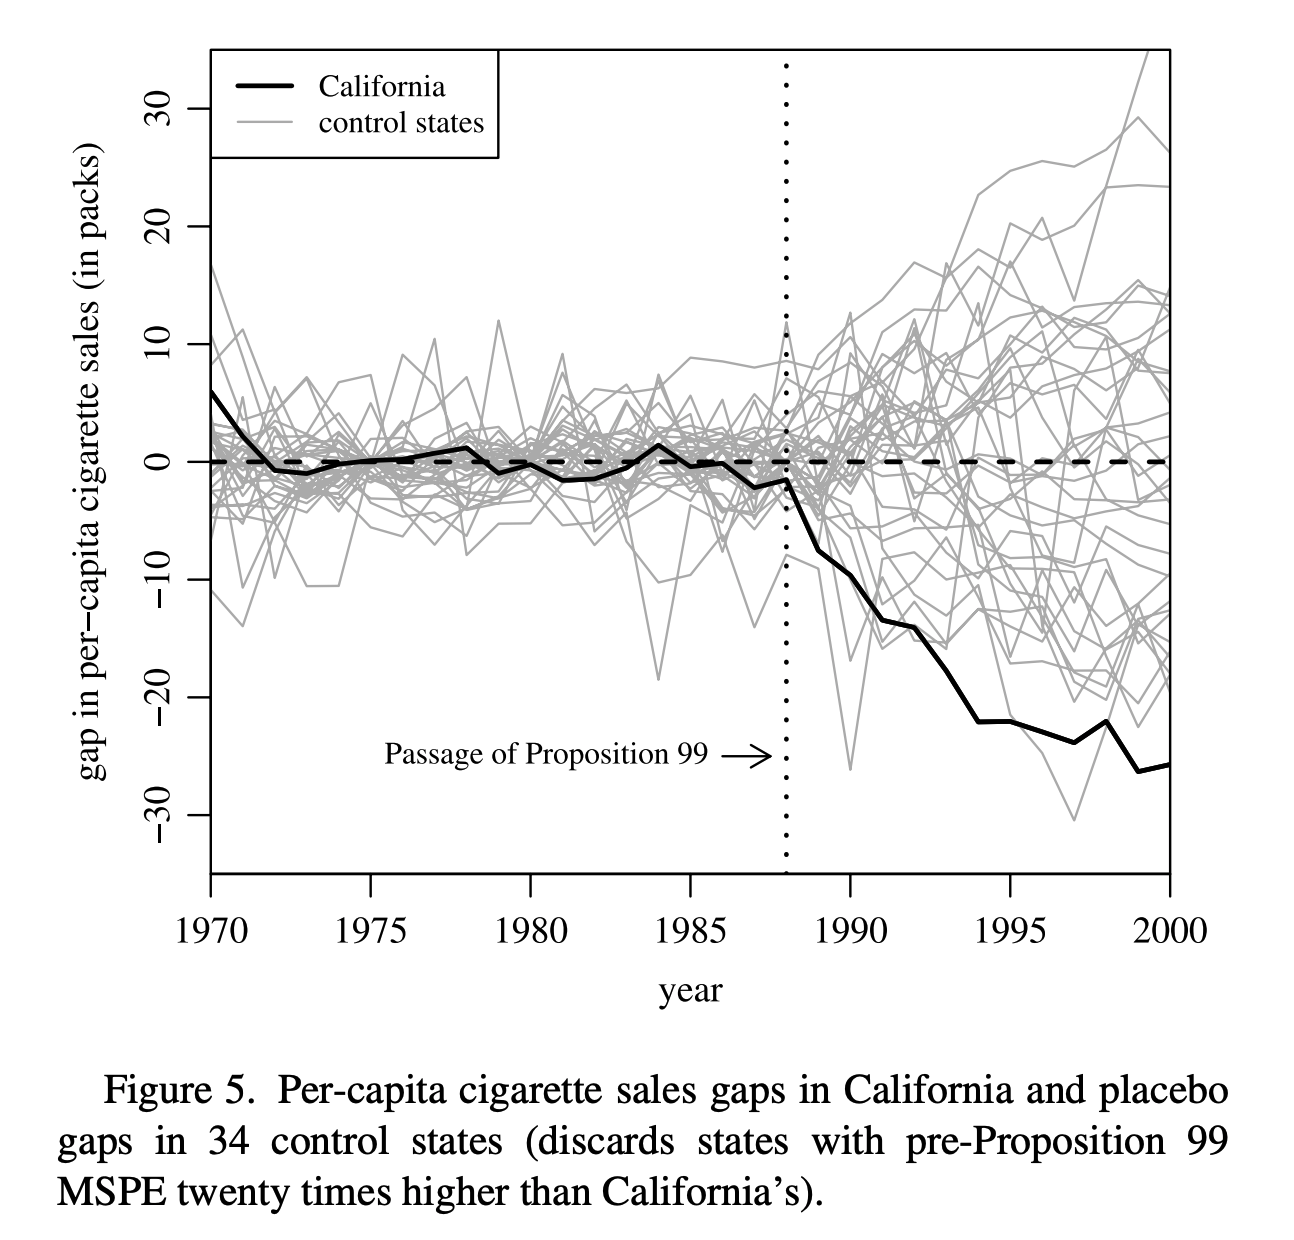
\includegraphics[width=\linewidth]{images/abadie2010d.png}}
\end{column}
\end{columns}
\end{frame}

%% Synthetic DiD block (from 14_synthetic_dind.tex)

\begin{frame}{Synthetic Diff-in-diff}
  \begin{wideitemize}
  \item In Arkhangelsky et al. (2019), they show you can rewrite the synthetic control estimator as
    \begin{equation*}
      (\hat{\mu}, \hat{\gamma}, \hat{\tau}) = \arg\min_{\mu, \gamma, \tau}\sum_{i}\sum_{t}(Y_{it} - \mu - \gamma_{t} - D_{it}\tau)^{2}\hat{\omega}_{i},
    \end{equation*}
    subject to the $\hat{\omega}_{i}$ chosen via the SC approach
  \item Contrast that with DID:
    \begin{equation*}
      (\hat{\mu},\hat{\alpha}, \hat{\gamma}, \hat{\tau}) = \arg\min_{\mu, \gamma, \tau}\sum_{i}\sum_{t}(Y_{it} - \mu -\alpha_{i} - \gamma_{t} - D_{it}\tau)^{2}
    \end{equation*}
  \item They then propose a more robust approach, called Synthetic diff-in-diff, which estimates
    \begin{equation*}
      (\hat{\mu},\hat{\alpha}, \hat{\gamma}, \hat{\tau}) = \arg\min_{\mu, \gamma, \tau}\sum_{i}\sum_{t}(Y_{it} - \mu -\alpha_{i} - \gamma_{t} - D_{it}\tau)^{2}\hat{\omega}_{i}\hat{\lambda}_{t}
    \end{equation*}
  \item This approach relaxes the parallel trends assumption by requiring parallel trends in an underlying approximate factor structure
  \end{wideitemize}
\end{frame}

\begin{frame}{Synthetic Diff-in-diff}
  \begin{columns}[T] % align columns
    \begin{column}{0.5\textwidth}
  \begin{wideitemize}
  \item Key difference is twofold:
    \begin{enumerate}
    \item Pre-trend means do not need to match ``exactly''
    \item Weighting is not equivalent across all time periods
    \end{enumerate}
  \item Conceptually -- different ways to generate the counterfactual given a model
  \end{wideitemize}
\end{column}
\begin{column}{0.5\textwidth}
  \only<1>{  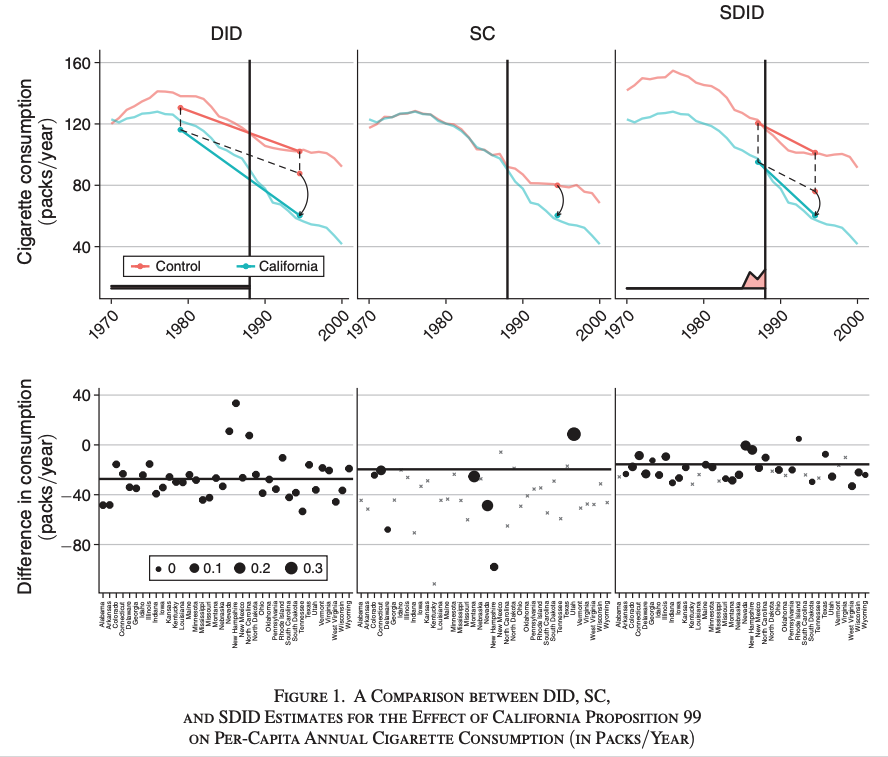
\includegraphics[width=\linewidth]{images/synthdid.png}}
  \only<2>{  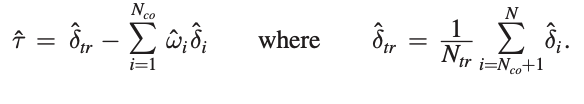
\includegraphics[width=\linewidth]{images/synthdid_eq1.png}\\
     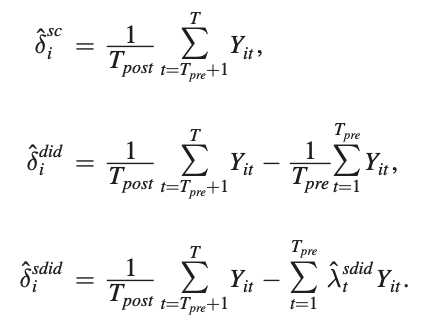
\includegraphics[width=\linewidth]{images/synth_eq2.png}}
\end{column}
\end{columns}
\end{frame}

\begin{frame}{Synthetic Diff-in-diff}
  \begin{columns}[T] % align columns
    \begin{column}{0.5\textwidth}
  \begin{wideitemize}
  \item So far, synth dind method discussion focused on single adoption period.
    \begin{enumerate}
    \item Staggered adoption in synthetic control isn't meaningful
    \item How can you adopt it?
    \end{enumerate}
  \item Conceptually -- split up the adoption timings a la Calloway \& Sant'anna and others
  \end{wideitemize}
\end{column}
\begin{column}{0.5\textwidth}
  \only<1>{  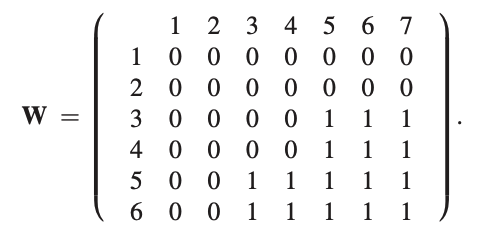
\includegraphics[width=\linewidth]{images/synthdid_staggered1.png}}
  \only<2>{  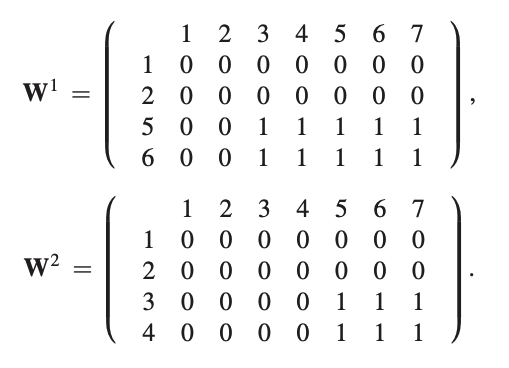
\includegraphics[width=\linewidth]{images/synthdid_staggered2.png}}
\end{column}
\end{columns}
\end{frame}


\begin{frame}{So what about synthetic methods?}
  \begin{wideitemize}
  \item Both an old field, and a new one -- lots of new methodological papers coming out
    \begin{itemize}
    \item It is a very cool method!
    \end{itemize}
  \item So far, limited application by researchers. Why?
  \item  My thoughts:
    \begin{itemize}
    \item These are strong structural assumptions, and not clear we
      have good tests yet
    \item Despite concerns re: pre-trends in dind, the assumptions
      felt testable
    \end{itemize}
  \item Researcher degrees of freedom seem multifold. True in DinD
    too, but perhaps more transparent?
    \begin{itemize}
    \item More worrisome: dind is equally problematic, but we aren't
      aware of it
    \end{itemize}
  \item If researchers are more willing to understand that DinD is
    sensitive to functional form, ML methods that construct
    counterfactual outcomes are a natural direction
  \end{wideitemize}
\end{frame}



\begin{frame}{My recommendation / takeaway}
  \begin{wideitemize}
  \item Synthetic control is the ideal approach when faced with a single treatment
    \begin{itemize}
    \item By far the most natural approach in this setting, and is a practical approach
    \item Typcial approach -- get a good synthetic control for a given
      treatment. If none exists, stop. Ben-Michael, Feller and
      Rothstein (2021) provide a better approach, which adjusts for
      imperfect pre-match.
    \end{itemize}
  \item Synthetic DiD seems very promising as a generalization
    \begin{itemize}
    \item Key question is convincing readers why this shoudl work better than traditional method
    \item My view: empirical papers will first need to show how / why
      their method works with both diff-in-diff and synth diff-in-diff
    \end{itemize}
  \item Key point: \emph{all of this relies on a model of the control outcome}
  \item Three packages to explore: augsynth/tidysynth andsynthdid
    packages (original synth package is tough to use)
  \end{wideitemize}
\end{frame}

%% Random timing (from 13_dind.tex + 14b_extensions_checklist.tex)

\begin{frame}{Taking a step back on design}
  \begin{columns}[T] % align columns
    \begin{column}{0.4\textwidth}
      \begin{wideitemize}
      \item The previous discussion all sits on the ``model-based'' approach for difference-in-differences
        \begin{itemize}
        \item E.g. Correctly modeling $E(Y(0))$ (the counterfactual)
        \item Challenging when thinking about logs vs. levels, for example
        \end{itemize}
      \item Alternative approach: random timing?
      \item<2-> Key point: we can define a propensity score where the treatment is considered ``random''
      \end{wideitemize}
    \end{column}%
    \hfill%
    \begin{column}{.5\textwidth}
      \only<1>{
\includegraphics[width=0.9\linewidth]{images/dind_randomtiming.png}}
      \only<2>{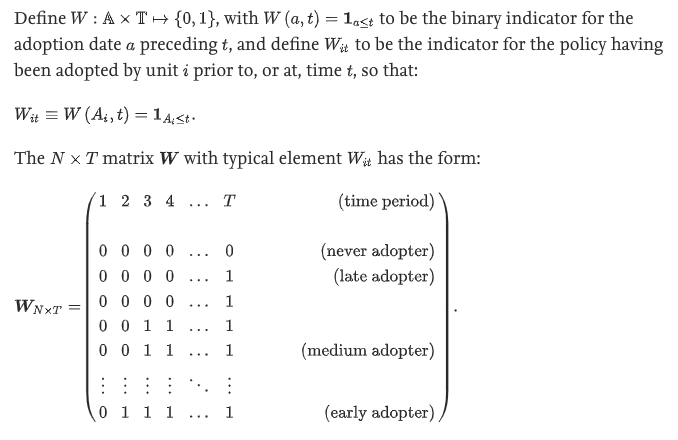
\includegraphics[width=0.9\linewidth]{images/dind_randomtiming2.png}}
    \end{column}
    \end{columns}
\end{frame}

\begin{frame}{Taking a step back on design}
  \begin{wideitemize}
  \item In the panel setting, it's worth considering whether you can just consider the policy ``as-if'' random, conditional on some controls
  \item Can you make units sufficiently comparable?
    \begin{itemize}
    \item E.g. if all firms greater than 100 employees are treated,
      could you compare firms just below 100 and just above 100 (to
      come in RD!)
    \item This would \emph{not} require a functional form assumption
    \end{itemize}
  \item Are there controls such that the groups appear ``observationally identical'' in the pre-period?
    \begin{itemize}
    \item Synthetic control + propensity score methods (to come)
    \end{itemize}
  \end{wideitemize}
\end{frame}

\begin{frame}{Random Timing in Diff-in-Diff}
  \begin{wideitemize}
  \item Athey and Imbens (2022) take design-based approach to diff-in-diff
    \begin{itemize}
    \item What does this mean? Can consider a well-defined propensity scores for the treatment
    \item Focus on staggered adoption with binary treatment
    \item Since treamtent is absorbing, this simplifies problem into ``when did I get the treatment (if ever)?''
    \end{itemize}
  \item E.g. define a propensity score: $Pr(A_{i} = a)$ over when the assignment occurs.
  \item Key question: who is the relevant counterfactual group?
  \end{wideitemize}
\end{frame}

\begin{frame}{Three key assumptions (not testable!)}
  \begin{enumerate}
  \item Random assignment (can make this happen by design)
  \item No anticipation (we assume this already)
  \item Invariance to history
    ($1_{a \leq t}(Y_{it}(a) - Y_{it}(1)) = 0$) (no causal effect of
    an early adotpion vs. a later adoption on outcome as long as
    adoption occured before or on period $t$)
  \end{enumerate}
\end{frame}

\begin{frame}{Efficiency in estimating staggered random roll-out}
  \begin{wideitemize}
  \item Roth and Sant'anna (2023) show that it is much more efficient
    to condition on lagged outcomes over using standard diff-in-diff
    in staggered roll-outs
  \item E.g. Consider the class of estimators:
    \begin{equation}
      \hat{\theta}_{\beta} = (\overline{Y}_{22} - \overline{Y}_{2\infty}) -  \beta(\overline{Y}_{12} - \overline{Y}_{1\infty})
    \end{equation}
    Did is the special case of $\beta=1$.
  \item We want to put more weight on this setting when the lagged
    outcomes are more predictive, and less when it is not!
    \begin{itemize}
    \item Intuition is similar to synthetic controls
    \end{itemize}
  \end{wideitemize}
\end{frame}

%% Covariates (from 14b_extensions_checklist.tex)

\begin{frame}{Covariates}
  \begin{wideitemize}
  \item With time-invariant covariates that treatment does not affect,
    controlling for covariates is conditional parallel trends
    assumption
    \begin{equation}
      E(Y_{i,2}(0)-Y_{i,1}(0) | D_{i} = 1, X_{i}) =       E(Y_{i,2}(0)-Y_{i,1}(0) | D_{i} = 0, X_{i})
    \end{equation}
  \item However, this isn't enough to satisfy this TWFE regression approach in two periods:
    \begin{equation}
      Y_{it} = \alpha_{i} + \phi_{t} + 1(t=2)D_{i}\beta + X_{i}1(t = 2)\gamma + \epsilon_{it}
    \end{equation}
    Why? (consider age)
  \item Even worse, if covariates affected by treatment, this is a form of
    collider bias!
    \begin{itemize}
    \item Should be very careful about time-varying covariates
    \end{itemize}
  \end{wideitemize}
\end{frame}

%% Multiple Treatments (from 14b_extensions_checklist.tex)

\begin{frame}{Multiple Treatments in Diff-in-diff}
  \begin{wideitemize}
  \item Hull (2018) and deChaisemartin and D'hautefeuille (2022) are relevant cites
  \item One ``easy'' context that this shows up (Hull 2018) is ``mover'' designs
    \begin{itemize}
    \item I move from city $i$ to city $j$ -- if my move was random,
      can we use it to understand the effect of city $j$?
    \item Without strong additional assumptions, challenging to
      interpret coefficients from standard TWFE
      \begin{equation}
        Y_{it} = \alpha_{i} + \tau_{t} + \sum_{j\not=0}\beta_{j}D_{ijt} + \epsilon_{it}
      \end{equation}
    \end{itemize}
  \item Consider 2 period case, and use first differences:
    \begin{equation}
      \Delta Y_{i} = \tau + \sum_{j\not=0}\beta_{j}\Delta D_{ij} + \Delta\epsilon_{i}
    \end{equation}
  \item Recall Goldsmith-Pinkham, Hull and Kolesar (2022) -- multiple
    treatments ($\Delta D_{ij}$) is potentially contaminated and
    negative weighted.
  \end{wideitemize}
\end{frame}

%% Continuous Treatment (from 14b_extensions_checklist.tex)

\begin{frame}{Fix ideas with example (Callaway, Goodman-Bacon, Sant'anna (2024))}
  \begin{center}
    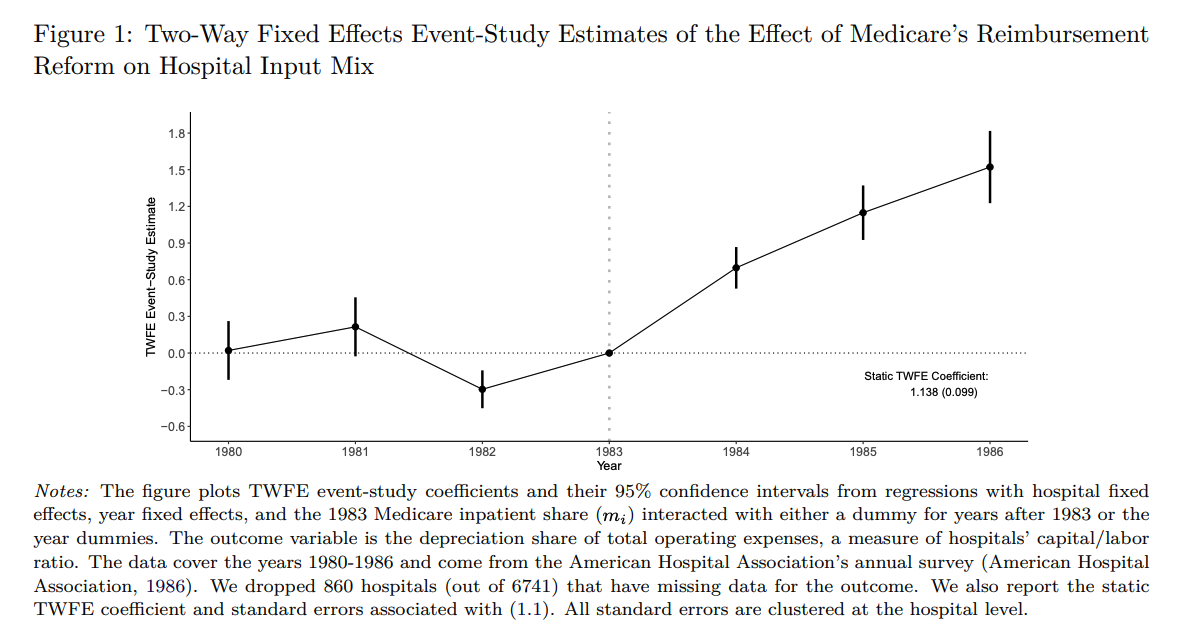
\includegraphics[width=0.75\linewidth]{images/continuous_did.png}
  \end{center}
  \begin{equation*}
    y_{it} = \theta_{t} + \eta_{i} + \beta D_{i} \cdot Post_{t} + \varepsilon_{it}
  \end{equation*}
  In 1983, Prospective Payment System changed payment for Medicare patients to hospitals
\end{frame}

\begin{frame}{Continuous treatment}
  \begin{wideitemize}
  \item Recall that estimating treatment effects with random
    assignment and continuous treatments was data hungry, but doable
  \item Without random assignment, and unconstrained heterogeneity,
    the challenge is more complicated
  \item First, consider what the estimand of interest is. Note that with potential outcomes, we now have $Y_{i}(D_{i})$ with $D_{i}$ multivalued.
  \item So what is the contrast of interest?
    \begin{align}
      ATT(d|d) &= E(Y_{i}(d) - Y_{i}(0) | D_{i} = d)\\
      ACRT(d|d) &= \frac{\partial E(Y_{i}(l) | D_{i} = d)}{\partial l}\bigg\rvert_{l = d}
    \end{align}
  \end{wideitemize}
\end{frame}


\begin{frame}{ACRT vs. ATT}
  \begin{center}
    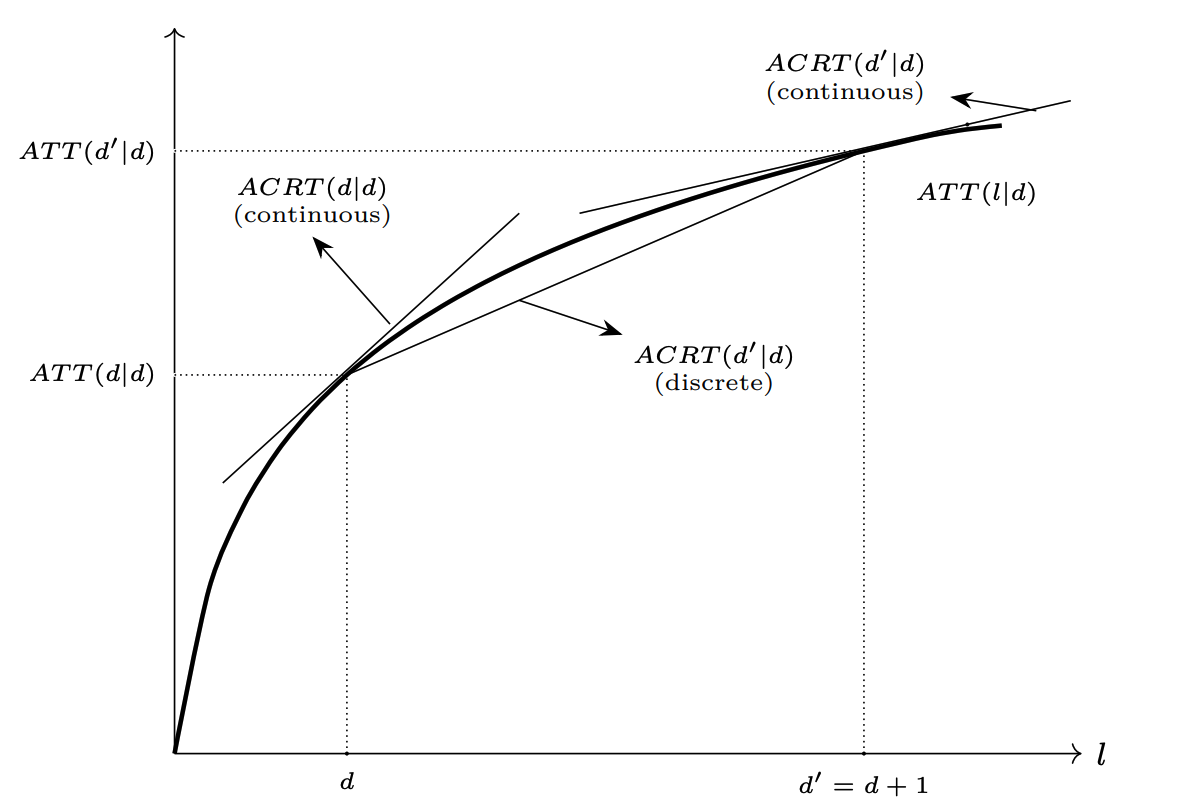
\includegraphics[width=0.75\linewidth]{images/acrt_1.png}
  \end{center}
\end{frame}



\begin{frame}{Continuous treatment -- Estimand}
  \begin{wideitemize}
  \item How do these differ? Consider their interpretations:
    \begin{itemize}
    \item ATT: effect relative to baseline of zero effect
    \item ACRT: effect of marginally increasing treatment, evaluted at a given point (can integrate too!)
    \end{itemize}
    \item Under parallel trends, what can we identify?
    \begin{itemize}
      \item First, parallel in what counterfactual? Under \emph{no} treatment
\begin{equation}
  E(Y_{2}(0) - Y_{1}(0) | D = d) = E(Y_{2}(0) - Y_{1}(0) | D = 0).
\end{equation}
implies
\begin{equation}
  ATT(d|d) = E(\Delta Y  | D = d) - E(\Delta Y | D = 0).
\end{equation}
    \end{itemize}
\item However, this does not identify anything about the ACRT

  \end{wideitemize}
\end{frame}

\begin{frame}{Continuous treatment -- Estimand}
  \begin{wideitemize}
    \item Can we move between ATT and ACRT?
    \item Under standard parallel trends,
    \begin{equation}
      \frac{\partial E(\Delta Y | D = d)}{\partial d} = \frac{\partial ATT(d|d)}{\partial d} = ACRT(d|d) + \frac{\partial ATT(d|l)}{\partial l}|_{l=d}
    \end{equation}
  \item Consider comparing two ATTs:
    \begin{align*}
      ATT(d | d) -  ATT(d' | d') &= \left(E[\Delta Y | D = d]  - E[\Delta Y | D=0]\right)\\
                                 &- \left(E[\Delta Y | D = d']  - E[\Delta Y | D=0]\right)\\
                                 &= E[\Delta Y | D = d]  - E[\Delta Y | D = d']\\
                                 &= E[\Delta Y(d) - \Delta Y(d') | D = d]  + ATT(d' | d) - ATT(d' | d')
    \end{align*}
  \end{wideitemize}
\end{frame}

\begin{frame}{Continuous treatment -- challenge}
  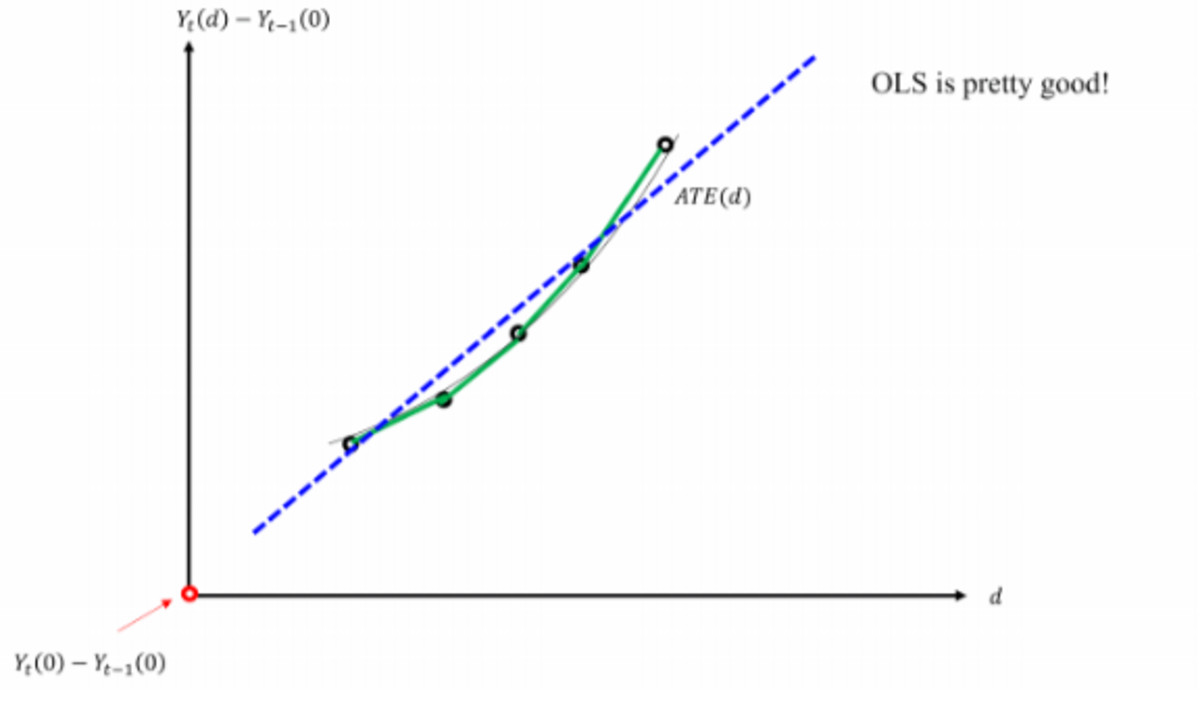
\includegraphics[width=0.8\linewidth]{images/continuous_did_1.pdf}
\end{frame}

\begin{frame}{Continuous treatment -- challenge}
  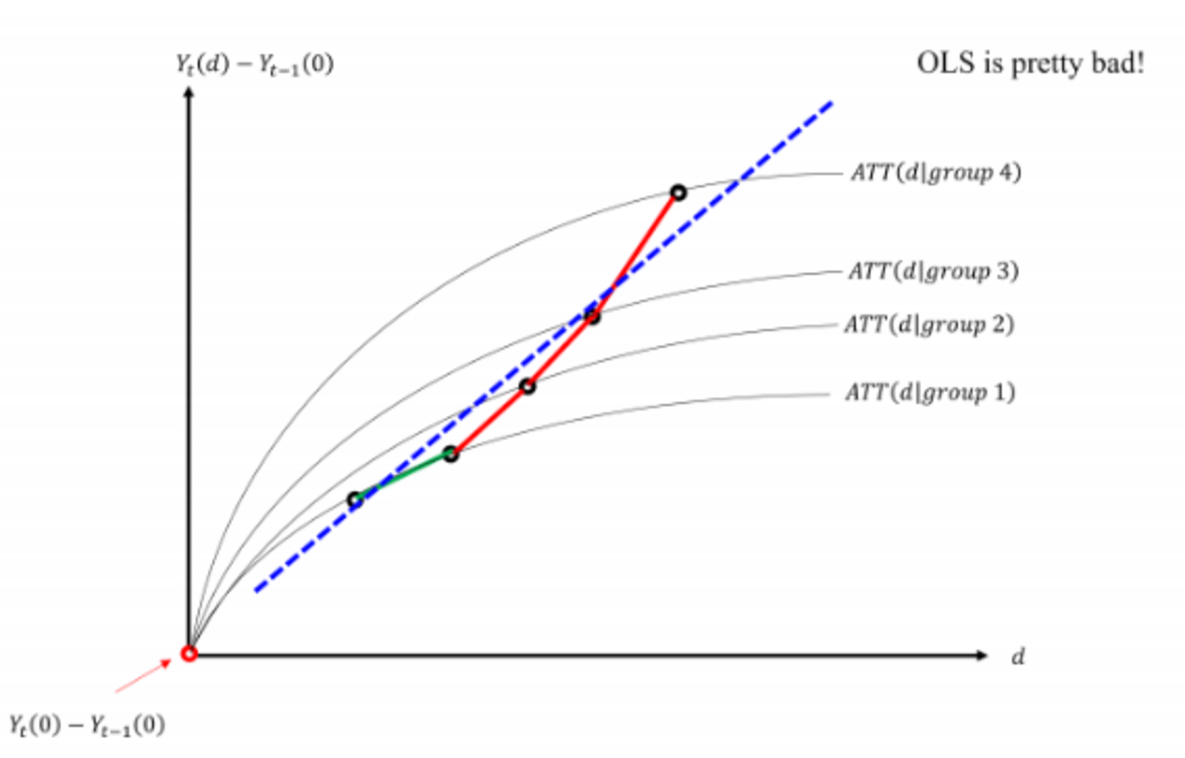
\includegraphics[width=0.8\linewidth]{images/continuous_did_2.pdf}
\end{frame}

\begin{frame}{Continuous treatment -- stronger assumption about heterogeneity}
  \begin{wideitemize}
  \item ``Strong'' parallel trends assumption: $E(\Delta Y_{i}(d)) = E(\Delta Y_{i}(d) | D_{i} = d)$
  \item No selection bias ``on average''
  \item Effectively assuming some kind of homogeneity in the treatment across groups
  \item Under this set of assumptions, you can identify the ATE as well as the ATT (and the ACR along with the ACRT)
  \end{wideitemize}
\end{frame}


\begin{frame}{Continuous treatment -- what if there is no untreated group?}
  \begin{wideitemize}
  \item Can consider parallel trends relative to some $d_{l}$ ``baseline'' group
  \item However, this mixes the selection effect based on treatment:
\begin{equation}
  E(\Delta Y | D_{i} = d) - E(\Delta Y | D_{i} = d_{l}) = ATT(d | d) - ATT(d_{l} | d_{l})
\end{equation}
and would need that $ATT(d_l|d) = ATT(d_{l}| d_{l})$ to identify the ATT
  \end{wideitemize}
\end{frame}

\begin{frame}{So what does TWFE do?}
  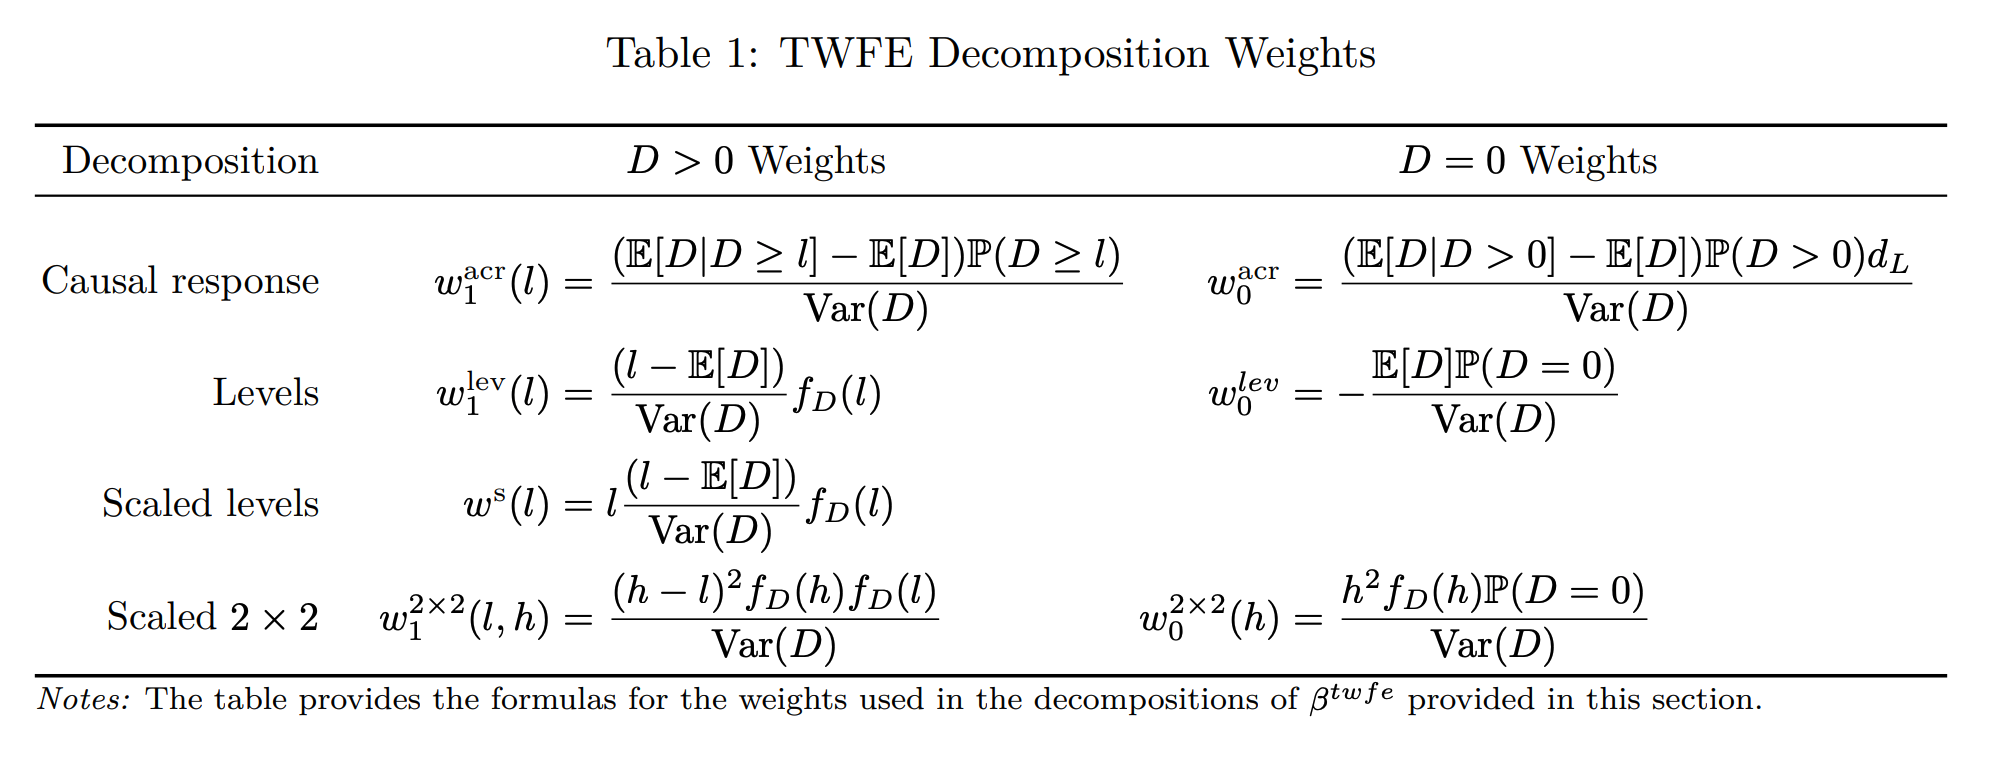
\includegraphics[width=0.8\linewidth]{images/twfe_continuous_did_weights.png}
  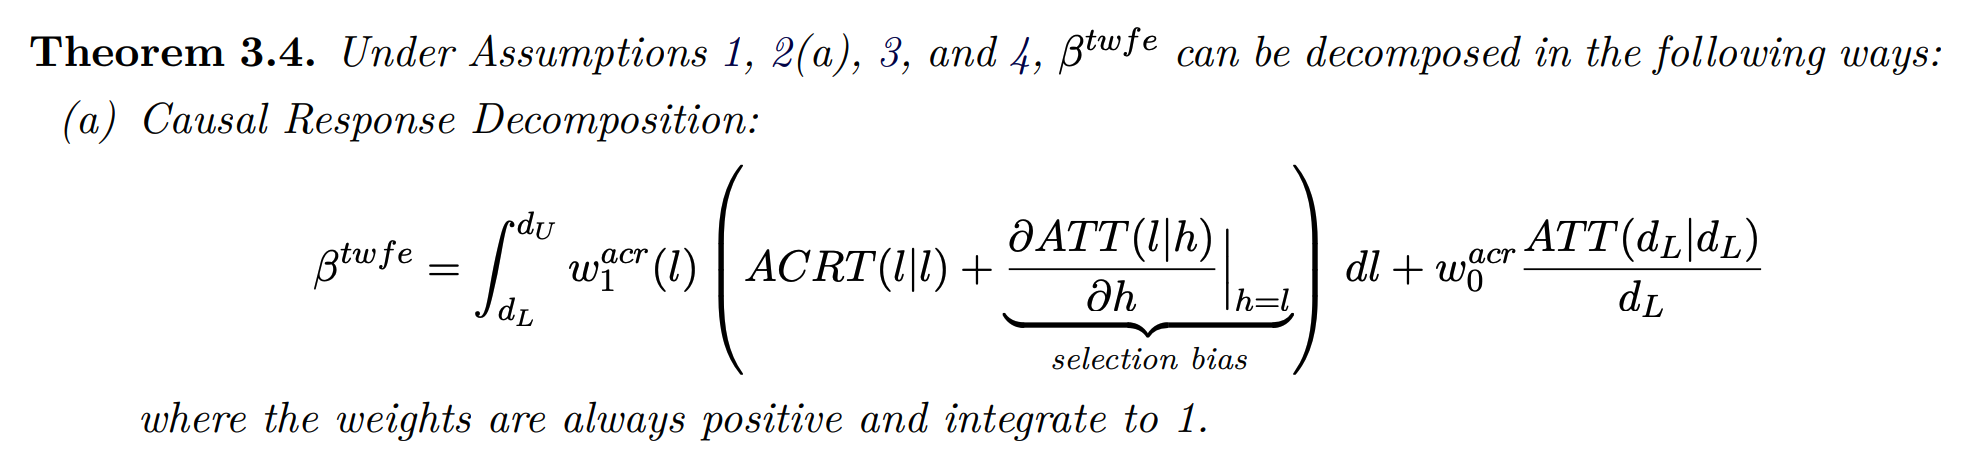
\includegraphics[width=0.8\linewidth]{images/twfe_continuous_did_formula1.png}

\end{frame}

\begin{frame}{So what does TWFE do?}
  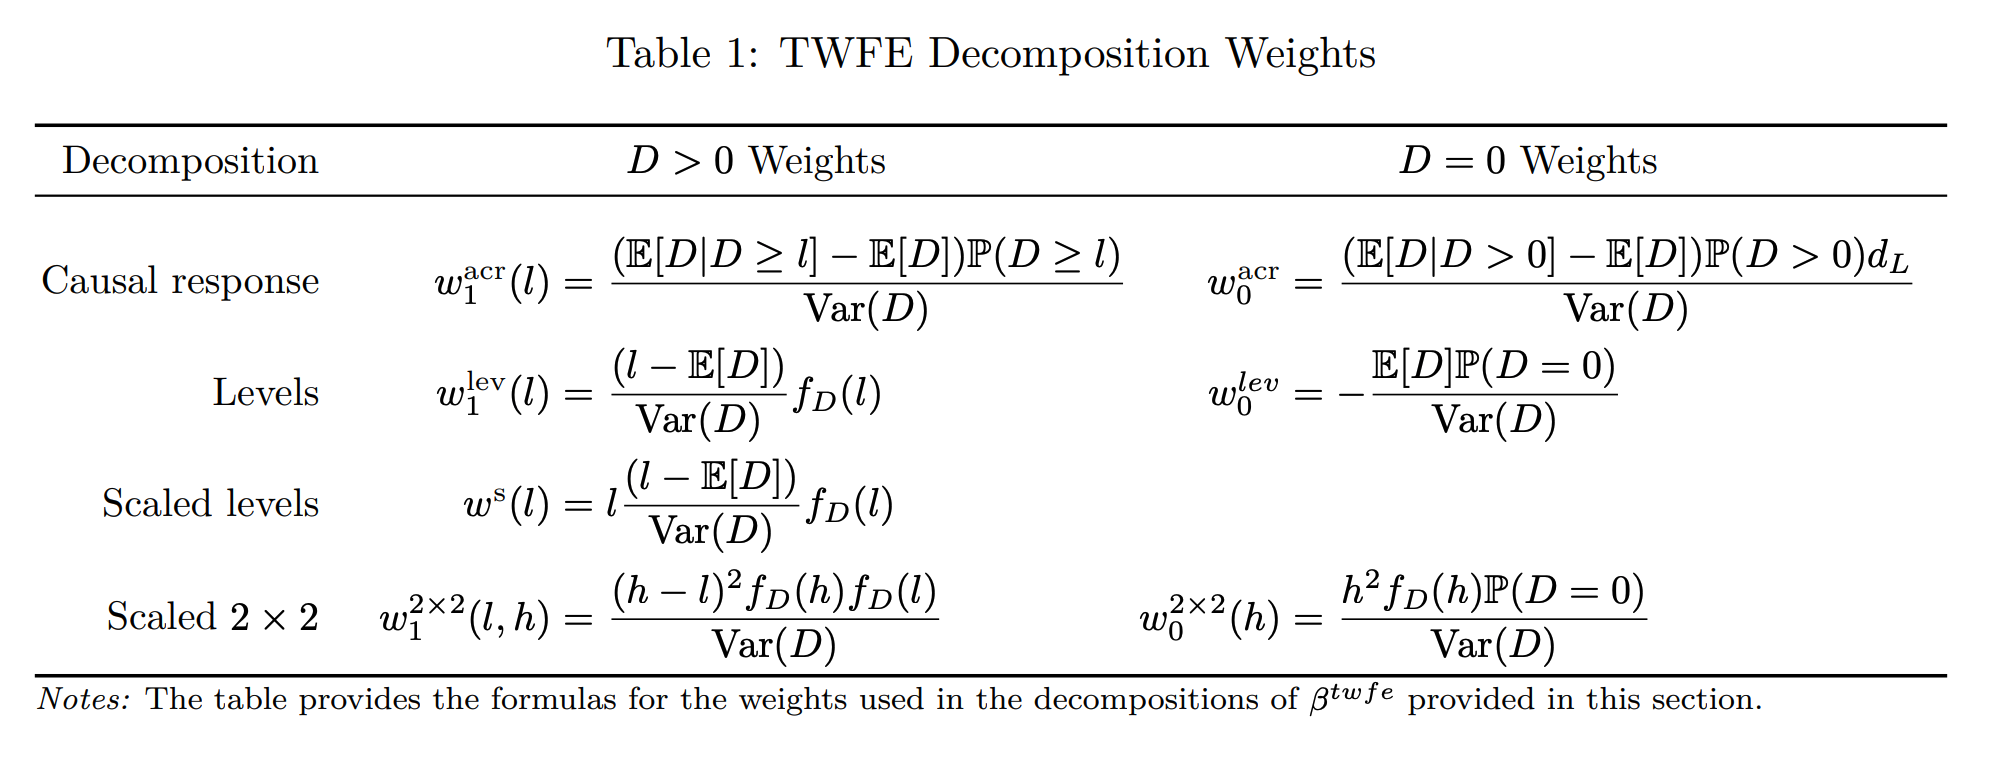
\includegraphics[width=0.8\linewidth]{images/twfe_continuous_did_weights.png}
  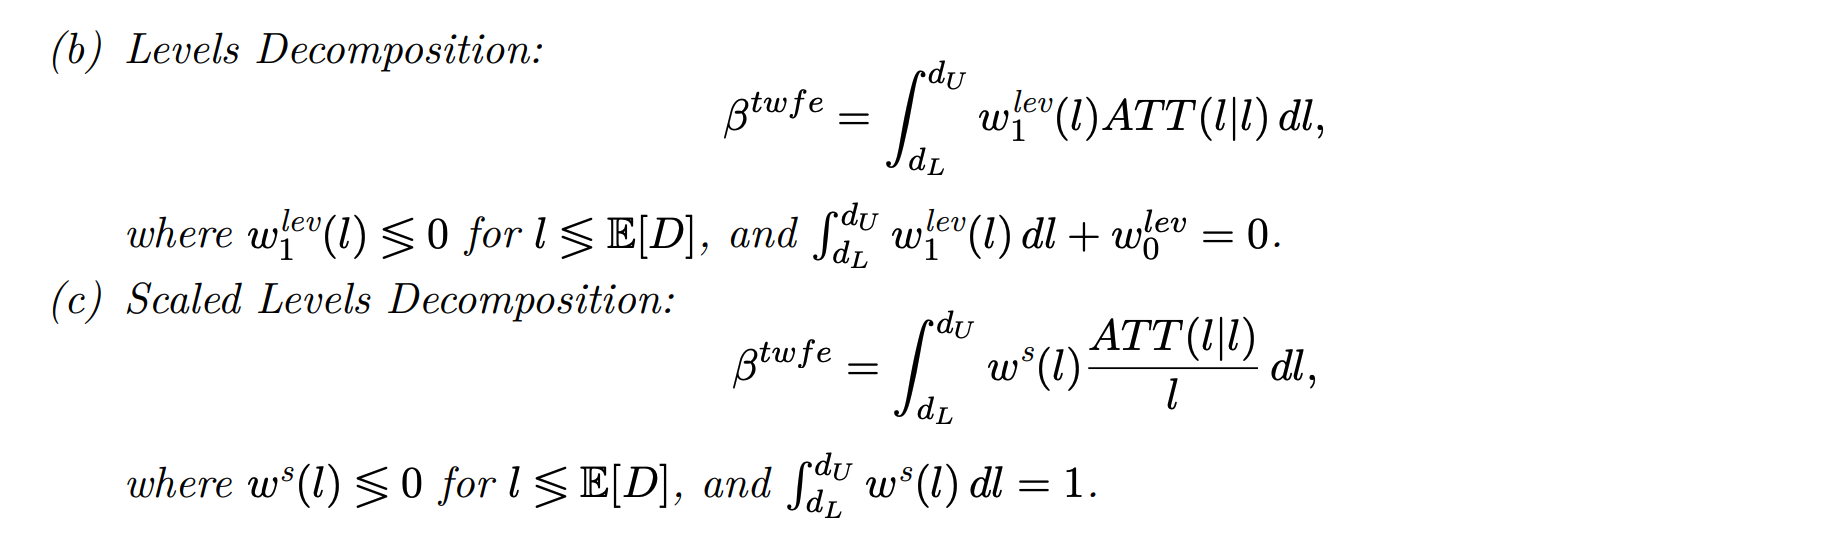
\includegraphics[width=0.8\linewidth]{images/twfe_continuous_did_formula2.png}
\end{frame}

\begin{frame}{Under strong parallel trends, TWFE gets convex ACR}
  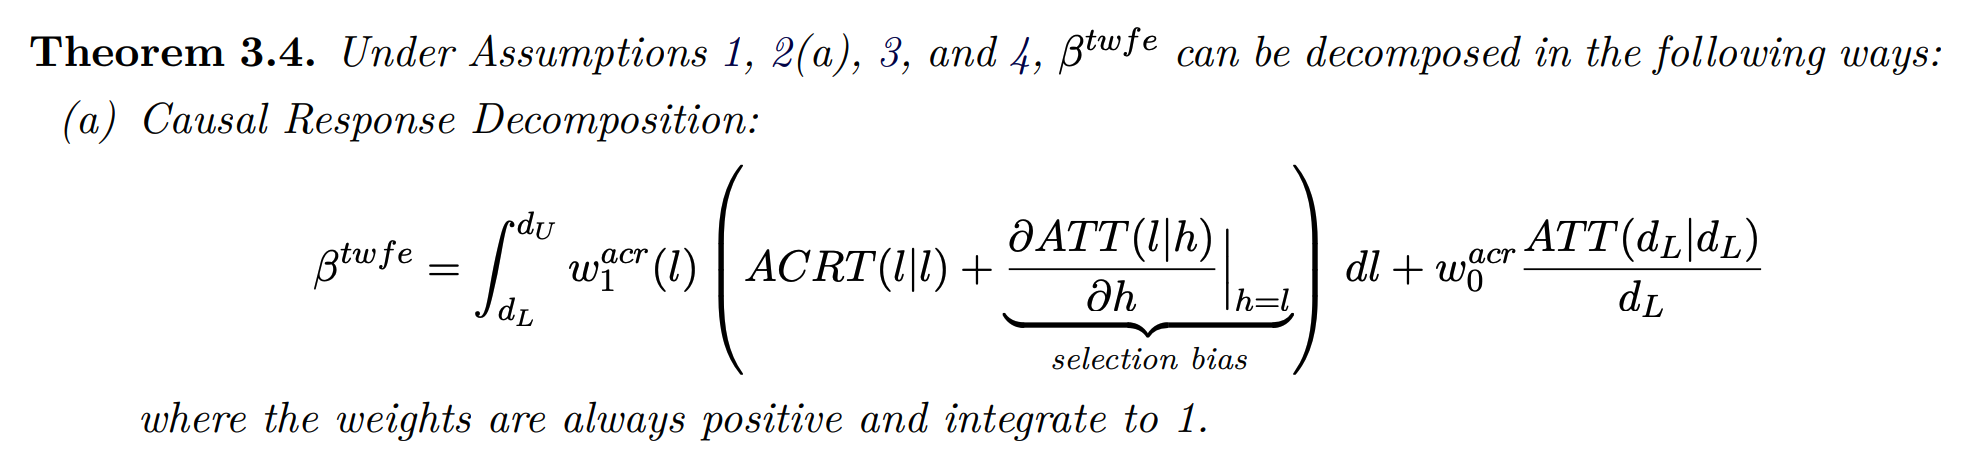
\includegraphics[width=0.8\linewidth]{images/twfe_continuous_did_formula1.png}
  \begin{wideitemize}
    \item Under strong parallel trends, the selection bias terms disappear (and with $d_{l} = 0$, last term disappears in (a))
    \item Weights are also convex and weakly causal! However, don't necessary map to an estimand of interest. Related to OLS weights from previous discussions
    \item ATT composition does not have convexity property
  \end{wideitemize}
\end{frame}

\begin{frame}{So what can you do?}
  \begin{wideitemize}
    \item Easiest thing is to use untreated units as baseline category
    \item When treatments are discrete:
    \begin{equation}
      \Delta Y_{i} = \beta_{0} + \sum_{j}1(D_{i} = d_{j})\beta_{j} + \epsilon_{i}
    \end{equation}
    Under parallel trends, each $\beta$ is $ATT(d|d)$, and with strong parallel trends, $\beta_{j} - \beta_{j-1}$ is $ACR(d_{j})$.
    \item Life is more complicated when $d$ is continuous of the groups are quite small at a given treatment:
    \begin{equation}
      \Delta Y_{i} = \sum_{k}\Psi_{Kk}(D)\beta_{Kk} + \epsilon_{i},
    \end{equation}
    where $\Psi_{Kk}(D)$ is a basis function for the treatment (implementation can be found in paper)
  \end{wideitemize}
\end{frame}

%% Checklist (from 14b_extensions_checklist.tex)

\begin{frame}{Checklist}
  \begin{wideitemize}
  \item First, consider the treatment features of your setup
      \begin{itemize}
    \item What is your treatment? Binary or continuous?
    \item Single or multiple?
    \item Absorbing or not?
    \item How many treated units? Single or many?
    \item How many interventions? Single or staggered timing?
    \end{itemize}
  \item Second, consider the relevant identifying assumptions for your condition
  \item Third, what tests are feasible in your setting?
  \item Fourth, what estimates do you want?
  \item Fifth, what relaxations of assumptions can you make?
  \end{wideitemize}
\end{frame}

\begin{frame}{Treatment features}
  \begin{wideitemize}
  \item If treatment is binary or only a few values, easy to consider the simple case
    \begin{itemize}
    \item Particularly helps if it's absorbing!
    \end{itemize}
  \item If continuous and/or not absorbing, need to worry about many more homogeneity assumptions
  \item First order of business -- \emph{define your estimand}.
    \begin{itemize}
    \item What treatment do you care about?
    \end{itemize}
  \item Can you simplify the problem in some way if it's more complex?
  \end{wideitemize}
\end{frame}

\begin{frame}{Assumptions}
  \begin{wideitemize}
  \item Write out carefully in math and then words what assumptions you need
    \begin{itemize}
    \item Parallel trends (with or without covariates)?
    \item No anticipation?
    \item Others?
    \end{itemize}
  \item If you know your estimand, much easier to know what you need
  \item Do you need to construct your estimator using lagged outcomes, e.g. synthetic control?
  \end{wideitemize}
\end{frame}

\begin{frame}{Testable assumptions}
  \begin{wideitemize}
  \item What is testable? Pre-trends can be useful, but underpowered
  \item If using random timing, not much is testable
    \begin{itemize}
    \item But could look for balance across timing groups in exogeneous features
    \end{itemize}
  \end{wideitemize}
\end{frame}

\begin{frame}{What estimates do you want?}
  \begin{wideitemize}
  \item Do you need a long run effect? Short-run?
    \begin{itemize}
    \item Long-run effect relies \emph{heavily} on parametric
      extrapolation. Is it plausible?
    \end{itemize}
  \item Are you studying ATTs? CATTs? ACRTs?
  \end{wideitemize}
\end{frame}

\begin{frame}{Relaxation of assumptions?}
  \begin{wideitemize}
  \item What group comparaisons are you making for parallel trends?
  \item Could you assume random timing instead of parallel trends?
  \item Could you condition on lagged outcomes?
  \end{wideitemize}
\end{frame}

%% Conclusion (from 13_dind.tex)

\begin{frame}{Conclusion}
  \begin{wideitemize}
  \item Difference in difference is hugely powerful in applied settings
  \item Does not require random assignment, but rather implementation
    of policies that differentially impacts different groups and is
    not confounded by other shocks at the same time.
  \item Can be a great application of big data, with convincing graphs
    that highlight your application
  \item Also allows for partial tests of identifying assumptions
  \item Worth carefully thinking about what your identifying
    assumptions are in each setting, and transparently highlighting
    them.
  \item Important to note that this always identifies a
    \emph{relative} effect, and to aggregate, you will typically need
    a model and additional strong assumptions (see Auclert, Dobbie and
    Goldsmith-Pinkham (2019) for an example in a macro setting).
  \end{wideitemize}
\end{frame}

\begin{frame}{My takeaways from new literature}
  \begin{wideitemize}
  \item Beware weak tests of pre-trends. Consider using R\&R's
    partial identification tests to assess robustness of results.
  \item Do not worry about the new literature on staggered timings if you only have one rollout period!
  \item Think carefully about your estimand if you're using a staggered timing DinD -- what's your counterfactual in each case?
    \begin{itemize}
    \item Software exists for many of these papers. This is doable!
    \end{itemize}
  \item When plotting confidence intervals in event studies, you should plot uniform confidence intervals.
  \end{wideitemize}
\end{frame}
\end{document}